%%
%% At least 2 slides but plan extra slides for discussion
%%

%% 1 slide on you
\frame{\frametitle{CV}
\begin{block}{Education}
% 2 items max
\begin{itemize}
\item PhD in Signal Processing, French naval Academy Research Institute - France - 2014
\item MSc in Signal Processing, UBO-ENSTA-Telecom Bretagne - France - 2010
\item BE from the Lebanese University, 2010
\end{itemize}
\end{block}

\begin{block}{Research topics}
\begin{itemize}
\item Signal processing, filtering, underwater acoustics, source localisation ...
\item Recently: Machine learning and speaker diarization.
\end{itemize}
\end{block}

%\begin{block}{Scientific contributions}
%\begin{itemize}
%\item h-index (3) \url{https://scholar.google.ch/citations?user=aeIX3V0AAAAJ&hl=fr}
%\item 12 (journals and conference papers)
%\end{itemize}
%\end{block}
}

% 1 slide on 1 research topic
\frame{\frametitle{Research topic}
\begin{block}{Enhanced Online Speaker Diarization}
\begin{itemize}
\item Integrate the inherent temporal structure of interactions between speakers.
\item Adapt state-of-the-art techniques to speaker diarization (such as i-vectors and deep learning).
\item Explore supervised and unsupervised domain adaptation techniques.
\end{itemize}
\end{block}

%\begin{block}{Research question(s)}
%\begin{itemize}
%\item Is there any of the abovementioned ambitious objectives not feasable?
%\end{itemize}
%\end{block}

%\begin{block}{Findings / Results}
%No results yet.
%\end{block}
}

%\frame{\frametitle{Research topic}
%\vspace{-1.5cm}
%\begin{figure}[htbp]
%\begin{center}
%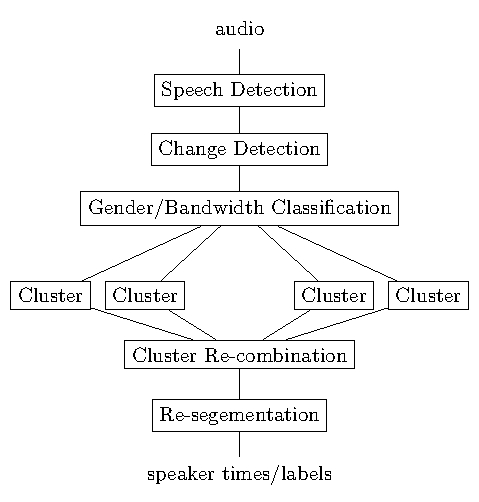
\includegraphics[width=0.65\textwidth]{Diagram_Speaker_diarization}
%\end{center}
%\caption{Prototypical speaker diarization system [Trantfer, 2006]}
%\label{Fig:Speaker_Rec}
%\end{figure}
%\vspace{-0.2cm}
%\scalebox{.4}{S. E. Tranter and D. A. Reynolds, "An overview of automatic speaker diarization systems," in IEEE Trans. on ASLP, vol. 14, no. 5, pp. 1557-1565, Sept. 2006.}

%}


% Additional slides for discussion
%\frame{\frametitle{Research topic}
%\begin{block}{...}
%\end{block}
%}


